\documentclass[border=2pt]{standalone}
\usepackage{tikz}
\usetikzlibrary{shapes.geometric}
\begin{document}
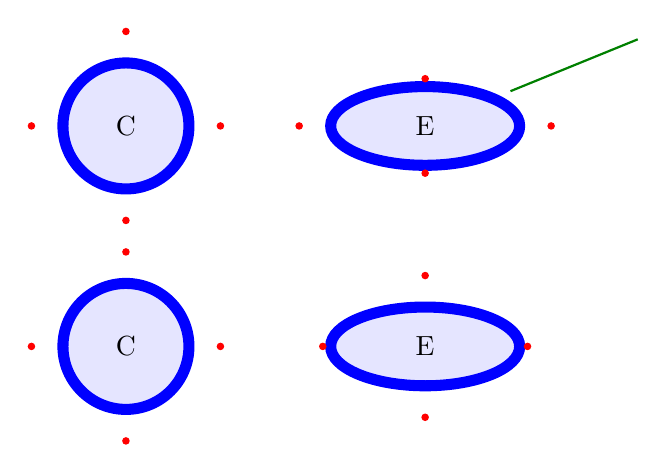
\begin{tikzpicture}[body/.style={draw=blue,fill=blue!10,line width=4pt,inner sep=0pt},
  wide/.style={outer xsep=4mm,outer ysep=1mm},tall/.style={outer xsep=1mm,outer ysep=4mm}]
  \node[body,circle,minimum size=16mm,wide] (cw) at (0,0) {C};
  \node[body,ellipse,minimum width=24mm,minimum height=10mm,wide] (ew) at (3.8,0) {E};
  \node[body,circle,minimum size=16mm,tall] (ct) at (0,-2.8) {C};
  \node[body,ellipse,minimum width=24mm,minimum height=10mm,tall] (et) at (3.8,-2.8) {E};
  \draw[green!50!black,line width=.8pt] (6.5,1.1) -- (ew);
  \foreach \n in {cw,ew,ct,et}{
    \foreach \a in {east,west,north,south}{
      \fill[red] (\n.\a) circle[radius=.48mm];
    }
  }
\end{tikzpicture}
\end{document}
